Die folgenden Abschnitte werden zuerst das Design des Spiels darlegen und einige der getroffenen Design-Entscheidungen erläutern und dann einen Überblick über die Implementation des Spiels liefern.

\subsection{Design}

% TODO: Deutscher Begriff
\subsubsection{Setting}

Diese Wahl des Settings birgt einige Vorteile.
Untote als Gegner zu verwenden erklärt sowohl die zwar Humanoiden, aber nicht unbedingt korrekt proportionierten, Ergebnisse des Creature Generators, als auch die zwar physikalisch basierten, aber nicht unbedingt natürlichen, Ergebnisse des Trainingsprozesses.

Kein Mitglied der Projektgruppe ist ein Erfahrener Künstler.
Für Texturen und Modelle wurden deshalb frei verfügbare Quellen verwendet.
Dieser Ansatz kann nicht mit der künstlerischen Kohärenz eines Teams von 3D-Modellierern, Grafikern, und Künstlern mithalten.
Die Dunkelheit des Settings hilft allerdings stark dabei dies zu kaschieren.

Einen Wald als Schauplatz zu verwenden erlaubt es das  Wissen über L-Systeme, dass sich in der Kreaturengenerierung als Sackgasse erwiesen hatte, weiter zu verwenden um prozedural Bäume zu generieren.

Die Wahl des Settings komplementiert somit die Ergebnisse der Projektgruppe und gleicht die Schwächen ihrer Mitglieder aus.

\subsubsection{Gameplay}
\label{sec:design-gameplay}
Wie zuvor erwähnt ist es die Aufgabe des Spielers sich vor den Untoten Kreaturen zu schützen.
Der Spieler verliert, wenn die Kreaturen ihn insgesamt dreimal berühren.
Der Spieler gewinnt, wenn er es schafft 10 Minuten lang nicht dreimal getroffen zu werden.

Der Spieler bekommt dafür zwei Werkzeuge
\begin{itemize}
    \item eine Taschenlampe, mit der er Kreaturen aus größerer Entfernung sehen kann,
    \item ein Gewehr, dass Kugeln verschießt, die sich auf etwa einen Meter Durchmesser aufblasen und an Oberflächen kleben bleiben.
\end{itemize}

Der Spieler muss das Gewehr nutzen um die ihn verfolgenden Kreaturen zu Fall zu bringen, zum Beispiel indem er genügend Kugeln auf die Kreatur schießt, dass diese unter dem Gewicht der Kugeln zusammenbricht.

Gefallene Kreaturen die sich einige Zeit lang nicht mehr nennenswerte Bewegen können sterben und werden aus dem Spiel entfernt.
Genauso entfernt das Spiel Kreaturen, die zu weit vom Spieler entfernt sind um noch Einfluss auf das Spiel zu haben.
Dafür werden an bestimmten, vom Terrain Generator festgelegten, Punkten regelmäßig neue Kreaturen erstellt, wobei das Spiel die Kreaturen möglichst nah am Spieler platziert, so dass der Spieler immer in Gefahr ist.

Das Gewehr nutzt elegant das Alleinstellungsmerkmal des Spiels aus, dass die Kreaturen durch ein neuronales Netz animiert werden.
Eine Kugel am Bein einer Kreatur zu platzieren ändert sichtlich ihr Bewegungsverhalten, da die Kreatur weiterhin versucht sich normal zu bewegen, was aber durch die zusätzliche Masse am Bein nicht gelingt.
Eine normale Animation würde dieses Verhalten nicht aufweisen.
Der Spieler kann also experimentieren, wie er sein Gewehr am effizientesten verwenden kann.

\subsubsection{Steuerung}

Das Spiel nutzt die konventionelle Steuerung für FPS-Spiele.
Der Spieler bewegt sich mit den WASD-Tasten und kontrolliert die Kamera mit der Maus. 
Tabelle \ref{tab:controls} zeigt die vollständige Tastenbelegung.

\begin{table}[]
    \centering
\begin{tabular}{c|c}
    Taste & Funktion \\
    W & Vorwärts\\
    A & Links\\
    S & Rückwärts\\
    D & Rechts\\
    Maus & Umschauen\\
    Links-Klick & Taschenlampe an/aus schalten, Schießen\\
    1 & Taschenlampe ausrüsten\\
    2 & Gewehr ausrüsten\\
    F12 & Screenshot
\end{tabular}
    \caption{Steuerung des Spiels}
    \label{tab:controls}
\end{table}

\begin{figure}
\centering
\begin{subfigure}[b]{0.75\textwidth}
   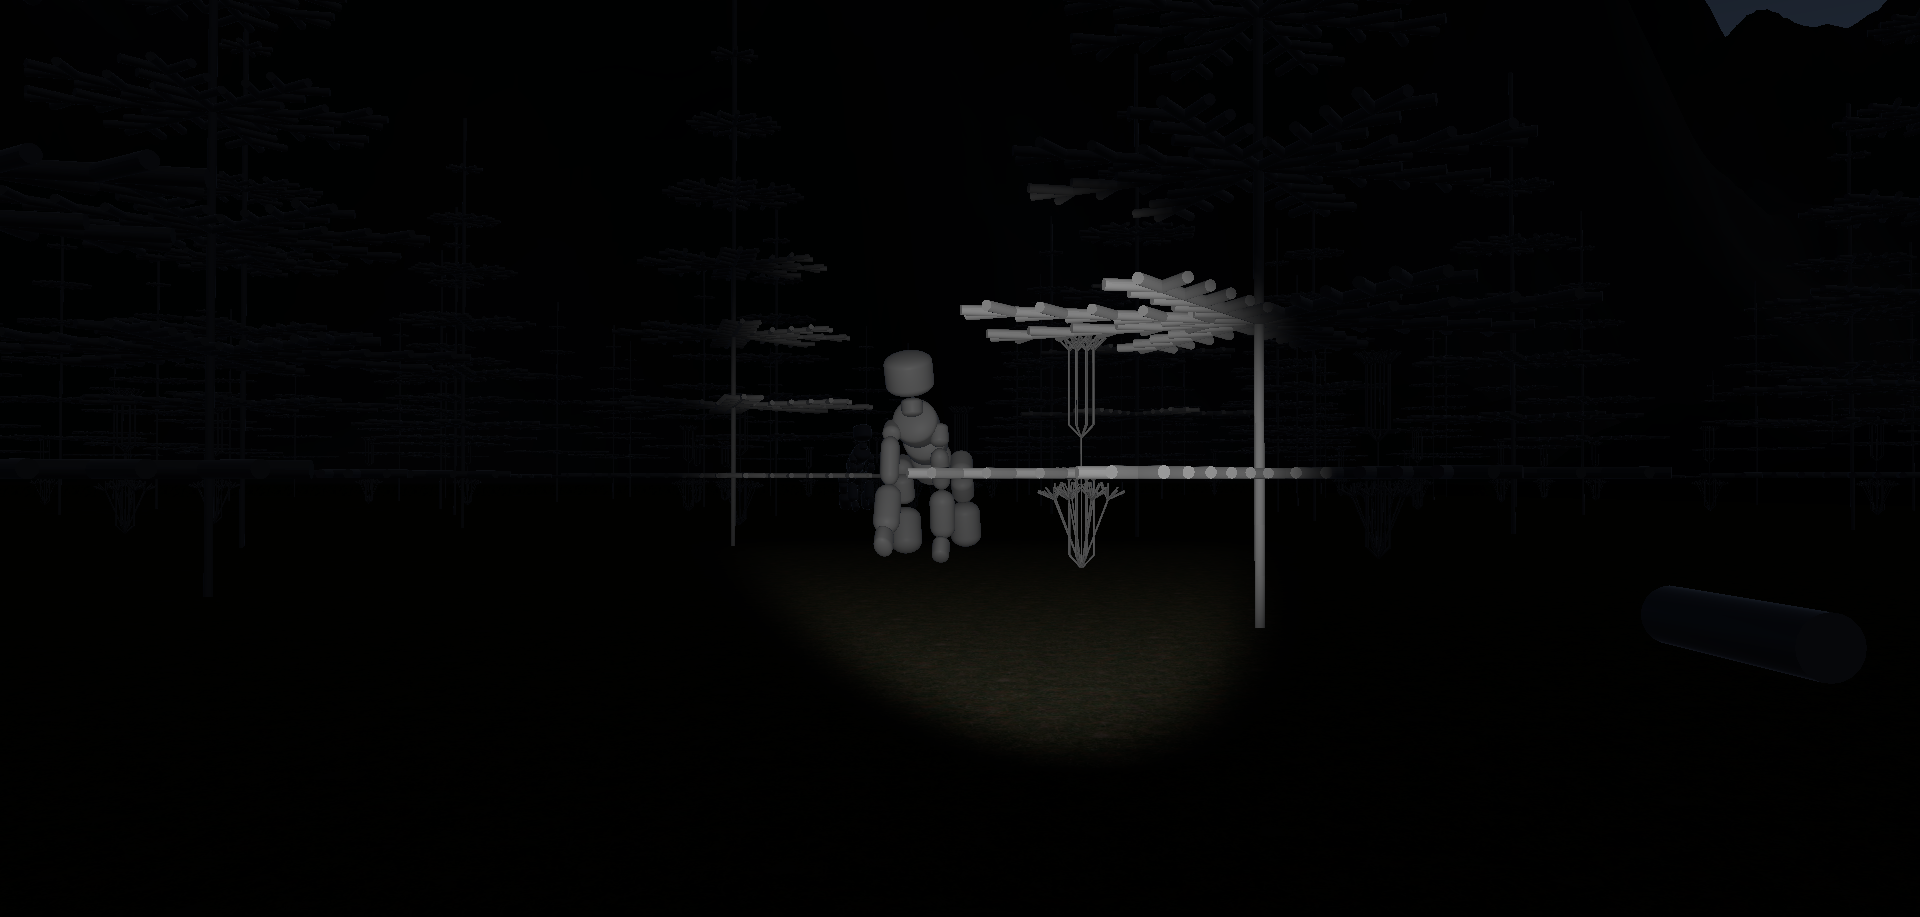
\includegraphics[width=1\linewidth]{resources/img/game_screenshot_1.png}
   \caption{Kreatur im dunklen Wald}
   \label{fig:game_screenshot_1} 
\end{subfigure}

\begin{subfigure}[b]{0.75\textwidth}
   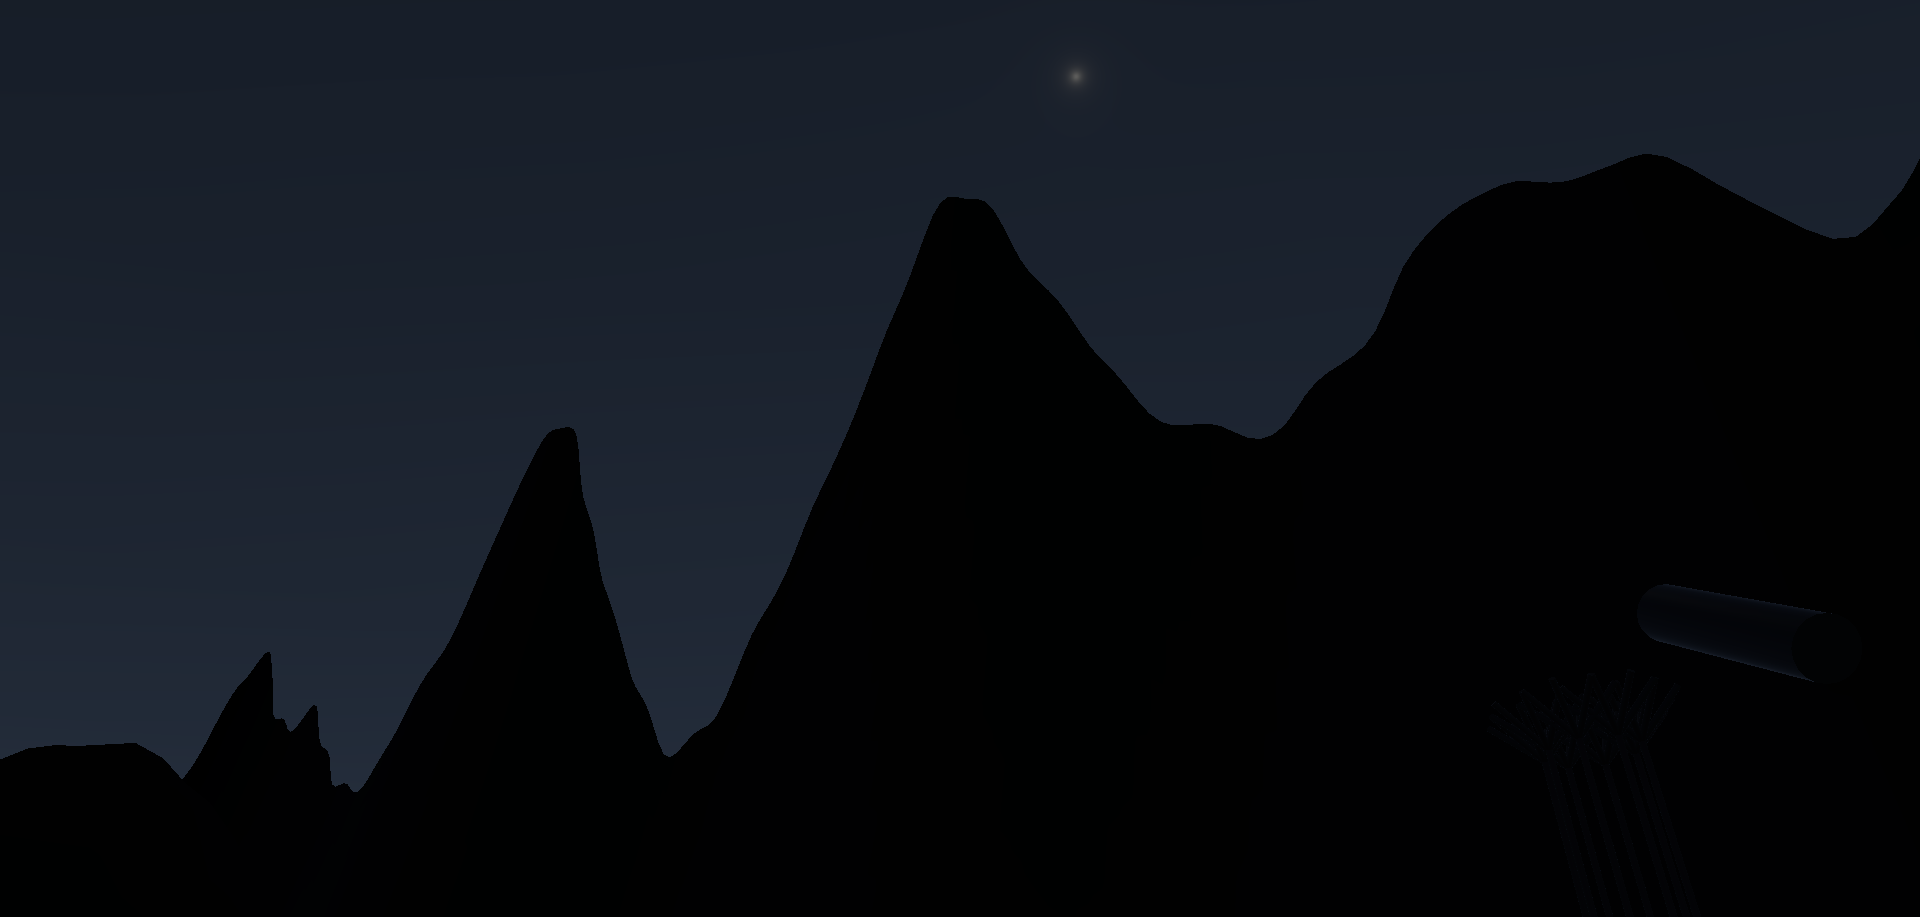
\includegraphics[width=1\linewidth]{resources/img/game_screenshot_2.png}
   \caption{Berge umgeben den Wald}
   \label{fig:game_screenshot_2}
\end{subfigure}

\begin{subfigure}[b]{0.75\textwidth}
   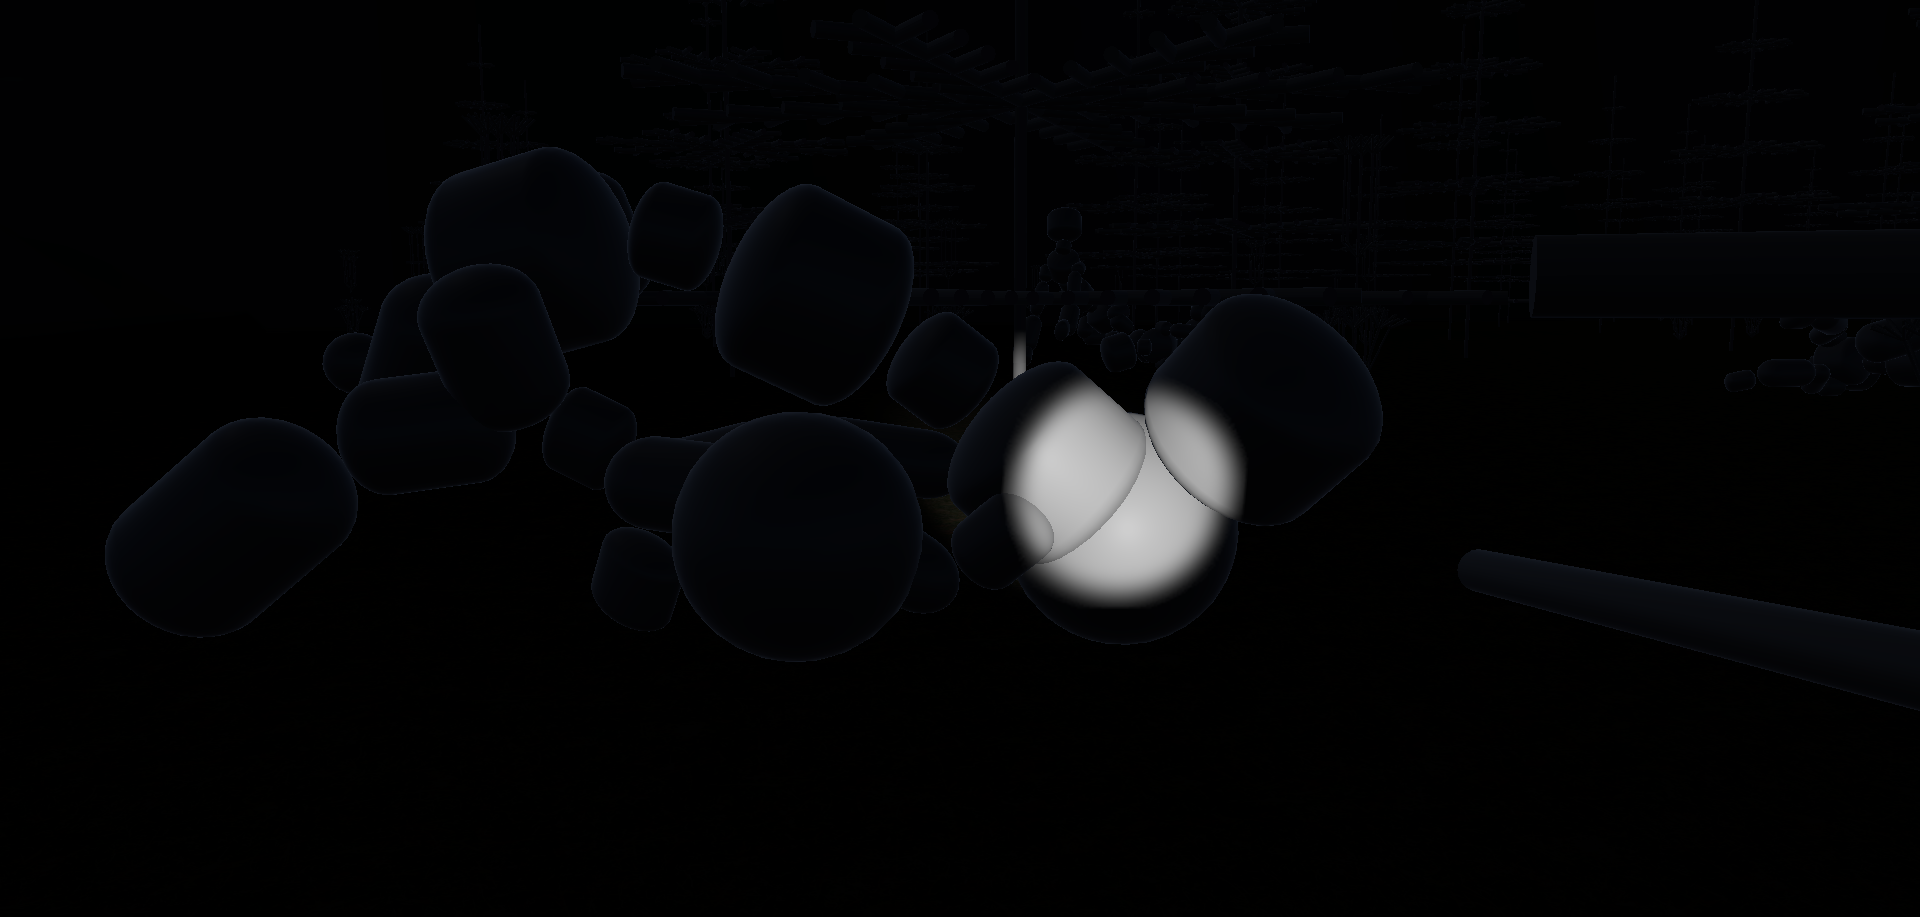
\includegraphics[width=1\linewidth]{resources/img/game_screenshot_3.png}
   \caption{Zu Fall gebrachte Kreatur}
   \label{fig:game_screenshot_3}
\end{subfigure}

\end{figure}

 
\subsection{Implementation}
Das Spiel besteht aus 5 Unity-Scenes.
Die \texttt{EntryPoint} Szene dient als Einstiegspunkt in das Spiel.
Die \texttt{Level} Szene enthält das eigentliche Spiel.
Die \texttt{LoadingScreen}, \texttt{GameOverScreen}, und \texttt{WinScreen} Szenen enthalten jeweils lediglich User Interfaces.

Die folgenden Abschnitte erläutern zunächst die Szenen genauer und gehen anschlißend genauer auf den Spielercharakter, die Kreaturen, und die Werkzeuge ein.

\subsubsection{EntryPoint}
Die Entrypoint Szene enthält drei \texttt{GameObject}s.

Das \texttt{Camera} Objekt enthält die eigentliche Kamera Komponente und das \texttt{CinemachineBrain}.
Dies ist die einzige Kamera im Spiel.
Alle weiteren Szenen werden Additiv zur \texttt{EntryPoint} Szene geladen und enthalten jeweils nur virtuelle Kameras.
So ist \texttt{Cinemachines} Invariante, dass nur eine nicht-virtuelle Kamera existieren darf, gesichert.

Das \texttt{Debug} Objekt enthält eine simple \texttt{DebugActions} Komponente, die das Erstellen von Screenshots mittels der F12 Taste ermöglicht.

Das \texttt{Init} Objekt enthält eine \texttt{Init} Komponente, die in ihrer Start-Methode den Szenenübergang zur \texttt{Level} Szene auslöst.
Der Übergang wird von der \texttt{SceneTransition} Klasse geleitet, die ebenfalls an dem \texttt{Init} Objekt anhängt.
Für den Szenenübergang werden zunächst additiv die \texttt{LoadingScreen} und \texttt{Level} Szenen geladen und die \texttt{Level} Szene wird als aktive Szene gesetzt.
Danach werden in einer Koroutine das Terrain generiert, Kreaturen generiert, und das Spielerobjekt erzeugt, wobei die Koroutine nach jedem Arbeitsschritt die Kontrolle abgibt, um das Spiel nicht einzufrieren.

\subsubsection{LoadingScreen, GameOverScreen, WinScreen}
Die drei UI Szenen sind identisch aufgebaut.
Sie enthalten jeweils ihre eigene virtuelle Kamera, ein \texttt{Input} Objekt mit einem \texttt{EventSystem} und dem \texttt{Input System UI Input Module}, und ein \texttt{UIDocument}.

\subsubsection{Level}
Die \texttt{Level} Szene enthält erneut eine virtuelle Kamera und ein direktionales Licht für die Szene.

Die \texttt{CreatureFactory} verwaltet die vom \texttt{CreatureGenerator} erzeugten Kreaturen.
Der \texttt{CreatureGenerator} produziert Bäume von \texttt{GameObjects}.
Da \texttt{GameObject}s immer Teil einer Szene sind, muss eine Prototyp Kreatur irgendwo in der Szene existieren, von der neue Kreaturen geklont werden können.
Die \texttt{CreatureFactory} verwaltet diese Prototypen und bietet Methoden zum erstellen neuer Kreaturen.
An dem \texttt{CreatureFactory} \texttt{GameObject} hängen außerdem Konfigurationsskripte, die ML-Agents Einstellungen beinhalten.

Das \texttt{SpawnManager} Skript ist für das Erzeugen und Entfernen von Kreaturen wie in Abschnitt \ref{sec:design-gameplay} beschrieben zuständig.
Dazu verwaltet es eine Liste von momentan aktiven Kreaturen.
In jedem Frame kontrolliert es zunächst ob Kreaturen sich selbst entfernt haben, dies kommt vor, wenn eine Kreatur bewegungsunfähig geworden ist.
Danach überprüft es für die verbliebenen Kreaturen, ob sie entfernt werden müssen, da sie zu weit vom Spieler entfernt sind, und erzeugt schließlich neue Kreaturen an den dem Spieler an nähesten liegenden Spawnpunkten.

Das \texttt{GameManager} Skript verwaltet die seit Spielstart vergangene Zeit und beendet das Spiel nachdem 10 Minuten vergangen sind.

\subsubsection{Spieler}
Der Spielercharakter ist als Prefab gespeichert und wird während des Ladevorgangs im Level platziert.
Es besteht aus einem Player \texttt{GameObject}, dass die für den Spielercharakter nötige Logik enthält, einer Kapsel als \texttt{Collider}, und zwei weiteren \texttt{GameObjects} die als Markierungen für die Positionen von Kamera und Werkzeugen dienen.

Das \texttt{Player} Objekt enthält die von Unity gestellten Komponenten \texttt{Character Controller} und \texttt{Player Input}, das Skript \texttt{Player Input State}, dass die von \texttt{Player Input} generierten Events erhält und so einen momentanen Eingabezustand verwaltet, und das Skript \texttt{FPSController}, was eine Weiterentwicklung des FPS Controllers aus Unitys FPS Template ist.

Der \texttt{FPSController} wurde um die Verwaltung des Lebenspunkte des Spielers und der Werkzeuge erweitert.
Um die Lebenspunkte zu verwalten wird ein Kollisionscallback im \texttt{FPSController} aufgerufen, wenn der Spieler mit den Knochen einer Kreatur kollidiert.
Das Verwalten der Werkzeuge erfolgt mittels eines \texttt{IEquipment} Interfaces, dass in Abschnitt \ref{sec:design-tools} genauer erläutert wird.

\subsubsection{Kreaturen}
Herz der Kreaturen Implementation ist das \texttt{BasicCreatureController} Skript.
Es ist dafür verantwortlich Pfade auf dem Navmesh zu finden und den jeweils nächsten Wegpunkt an die KI zu liefern.
Außerdem überwacht es die Geschwindigkeit der Kreatur an der es angebracht ist und entfernt sie aus dem Spiel, wenn sie sich zu lange nicht bewegt.
So wird verhindert, dass das Budget des \texttt{SpawnManager}s mit Bewegungsunfähigen Kreaturen verbraucht wird.
Das \texttt{BasicCreatureController} Skript wird in der \texttt{CreatureFactory} automatisch an neu erstellte Kreaturen gehangen.

\subsubsection{Werkzeuge}
\label{sec:design-tools}
Die Werkzeuge sind als Prefabs gespeichert.
Das oberste Objekt des Prefabs muss jeweils ein Skript besitzen, dass das \texttt{IEquipment} Interface implementiert.
Das Interface besitzt die 4 Methoden \texttt{OnPrimary}, \texttt{OnSecondary}, \texttt{OnEquip}, und \texttt{OnUnequip}, die vom \texttt{FPSController} aufgerufen werden.
Mit diesen Methoden können die Werkzeuge darauf reagieren, dass die linke, bzw. rechte, Maustaste gedrückt wurde, dass sie ausgerüstet wurden, und dass ein anderes Werkzeug ausgerüstet wurde.

Die Taschenlampe enthält ein \texttt{Spotlight}, dass beim Klicken der linken Maustaste an- und ausgeschaltet wird.

Das Gewehr enthält ebenfalls ein \texttt{Spotlight} für den Lichtkegel des Gewehrs.
Beim Klicken der Linken Maustaste führt das Gewehr einen Raycast von der momentanen Kamera aus und platziert ein \texttt{BallGunProjectile} an der so gefundenen Stelle.
Das \texttt{BallGunProjectile} spielt dann selbstständig seine Animationen ab und entfernt sich nach einiger Zeit selbst wieder aus der Szene.

Beide Werkzeuge reagieren auf \texttt{OnEquip}, \texttt{OnUnequip} damit sich selbst An- und Abzuschalten.